\chapter{Measurement of \kVV through VBS VVH production}
\begin{aquote}{Richard Feynman, The Feynman Lectures, 1963}
The principle of science, the definition, almost, is the following: The test of all knowledge is experiment. 
Experiment is the sole judge of scientific ``truth.''
\end{aquote}
\section{Motivation}
\begin{figure}[htb]
    \centering
    \subfloat{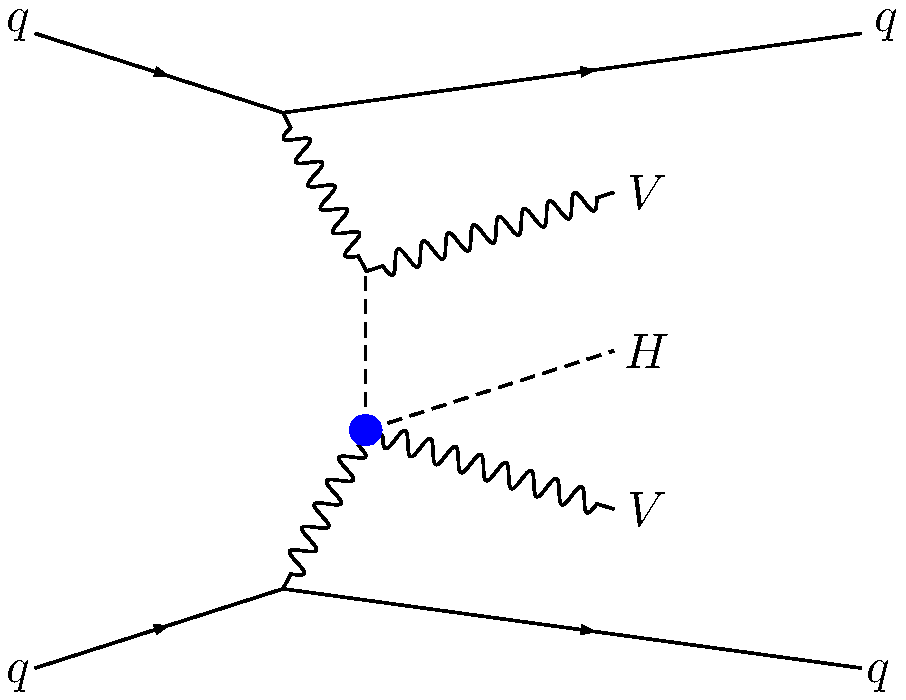
\includegraphics[width=0.3\textwidth]{fig/feynman/vbsvvh/vbsvvh_c2v.pdf}}\quad
    \subfloat{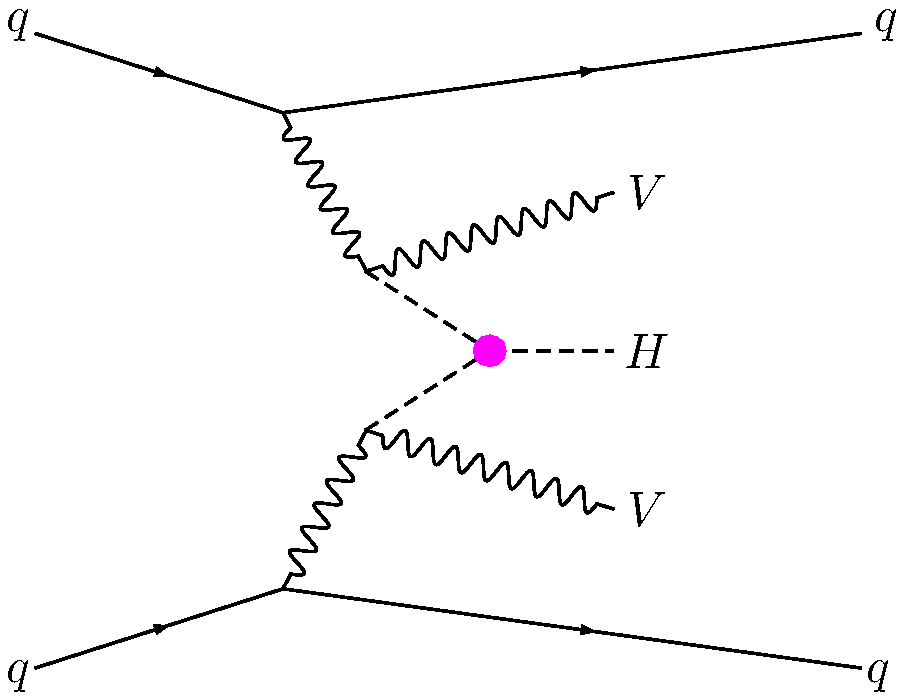
\includegraphics[width=0.3\textwidth]{fig/feynman/vbsvvh/vbsvvh_c3.pdf}}\quad
    \caption{
        Leading-order Feynman diagrams for VBS production of two vector bosons (V) and one Higgs boson. 
        The HHVV coupling \kVV is denoted by a blue circle (\textcolor{blue}{\ding{108}}), and the HHH coupling \kHHH is denoted by a magenta circle (\textcolor{magenta}{\ding{108}}). 
    }
    \label{fig:vbsvvh_feynman}
\end{figure}
\section{The signal}
\begin{figure}[htb]
    \centering
    \subfloat{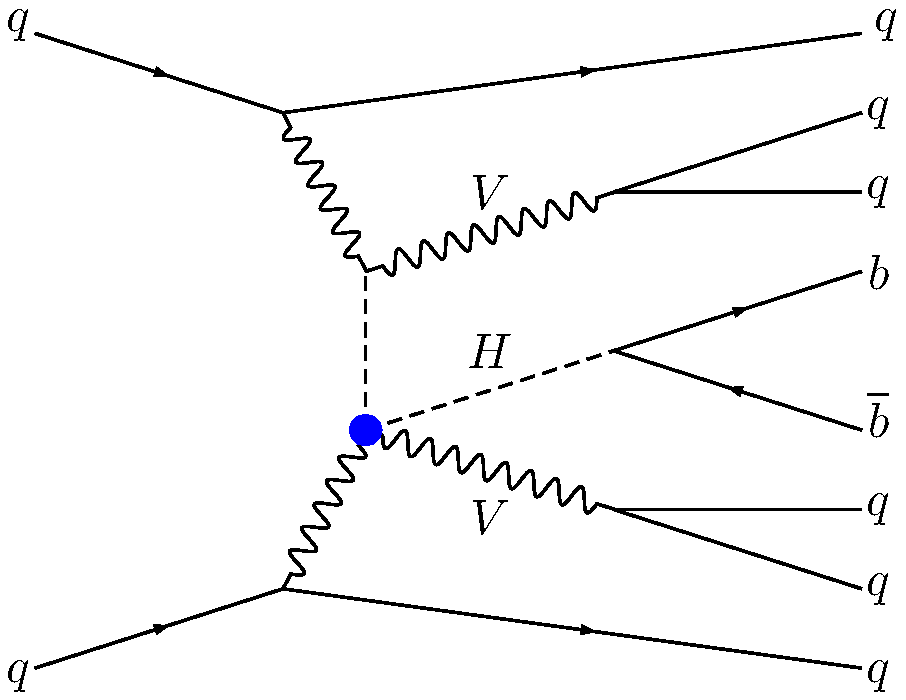
\includegraphics[width=0.3\textwidth]{fig/feynman/vbsvvh/vbsvvh_c2v_allhad.pdf}}\quad
    \subfloat{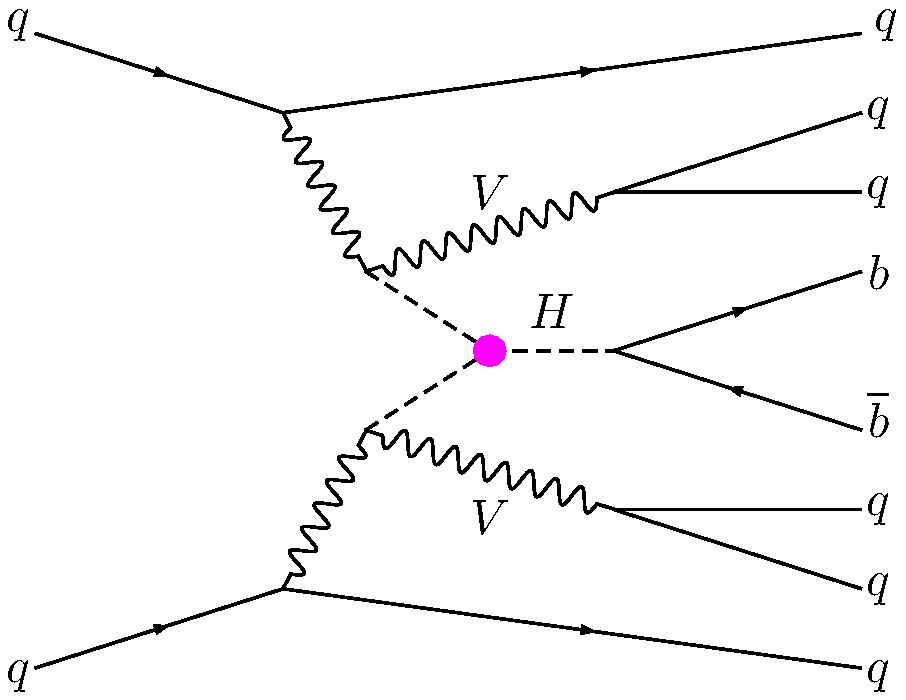
\includegraphics[width=0.3\textwidth]{fig/feynman/vbsvvh/vbsvvh_c3_allhad.pdf}}\quad
    \caption{
        Leading-order Feynman diagrams for VBS production of two vector bosons (V) and one Higgs boson, where the vector bosons decay hadronically and the Higgs boson decays specifically to b quarks. 
        The HHVV coupling \kVV is denoted by a blue circle (\textcolor{blue}{\ding{108}}), and the HHH coupling \kHHH is denoted by a magenta circle (\textcolor{magenta}{\ding{108}}). 
    }
    \label{fig:vbsvvh_feynman_allhad}
\end{figure}
\section{The backgrounds}
\section{Event selection}
\section{ABCDNet}
\section{Background estimation}
\section{Results}
